\documentclass{article}

\title{WMC Junior Finals Proof Questions - Set 2}
\author{Fredric Gregory King Chung}
\date{\today}

\usepackage{amssymb}
\usepackage{amsfonts}
\usepackage{amsmath}
\usepackage{graphicx}
\usepackage{float}
\usepackage[margin=1in]{geometry}

\begin{document}
\maketitle

\section{A Lesson in Invariants}

\noindent\textbf{Problem 1.} There is an $8 \times 8$ chessboard with two tiles missing, as indicated below.

\begin{figure}[H]
    \centering
    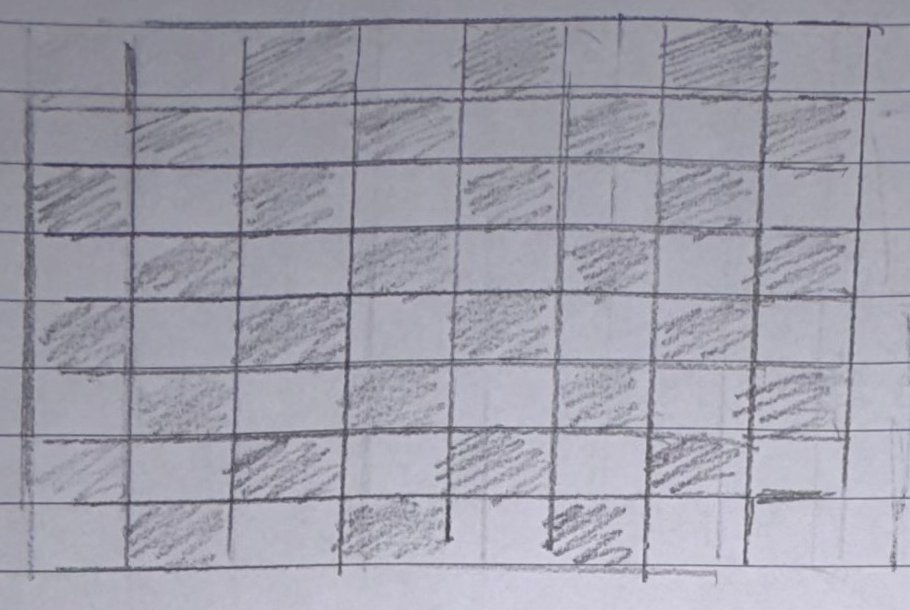
\includegraphics[width=0.5\textwidth]{figures/p1-fig-board.jpg}
\end{figure}

\noindent Prove that it is impossible to tile the board with $2 \times 1$ tiles.

\bigskip

\noindent\textbf{Solution 1.}

\medskip

\noindent\textbf{(a)} Note that any $2 \times 1$ tile will cover 1 white and 1 black square. Hence, any tiling of a chessboard with $2 \times 1$ tiles will cover an equal number of white and black squares.

\medskip

\noindent A normal chessboard has
\[
    \frac{1}{2}(8)(8) = 32
\]
white squares and 32 black squares. The modified board has 32 white squares, but only
\[
    32 - 2 = 30
\]
black squares: not equal.

\medskip

\noindent Hence, it is impossible to tile the board with $2 \times 1$ tiles. $\qquad \square$

\section{Trigonometry with Paper Folding}

\noindent\textbf{Problem 2.} By folding a square piece of paper, prove that
\[
    \tan^{-1} 1 + \tan^{-1} 2 + \tan^{-1} 3 = \pi.
\]
(\textbf{Hints:} Centroids split a median into the ratio $2:1$ (two-thirds and one-third). Can you use that to get $\tan^{-1} 3$? What kind of special right triangles have $\tan^{-1} 1$ and $\tan^{-1} 2$ as angles? Think about the ratio of sides.)

\bigskip

\noindent\textbf{Solution 2.}

\begin{figure}[H]
    \centering
    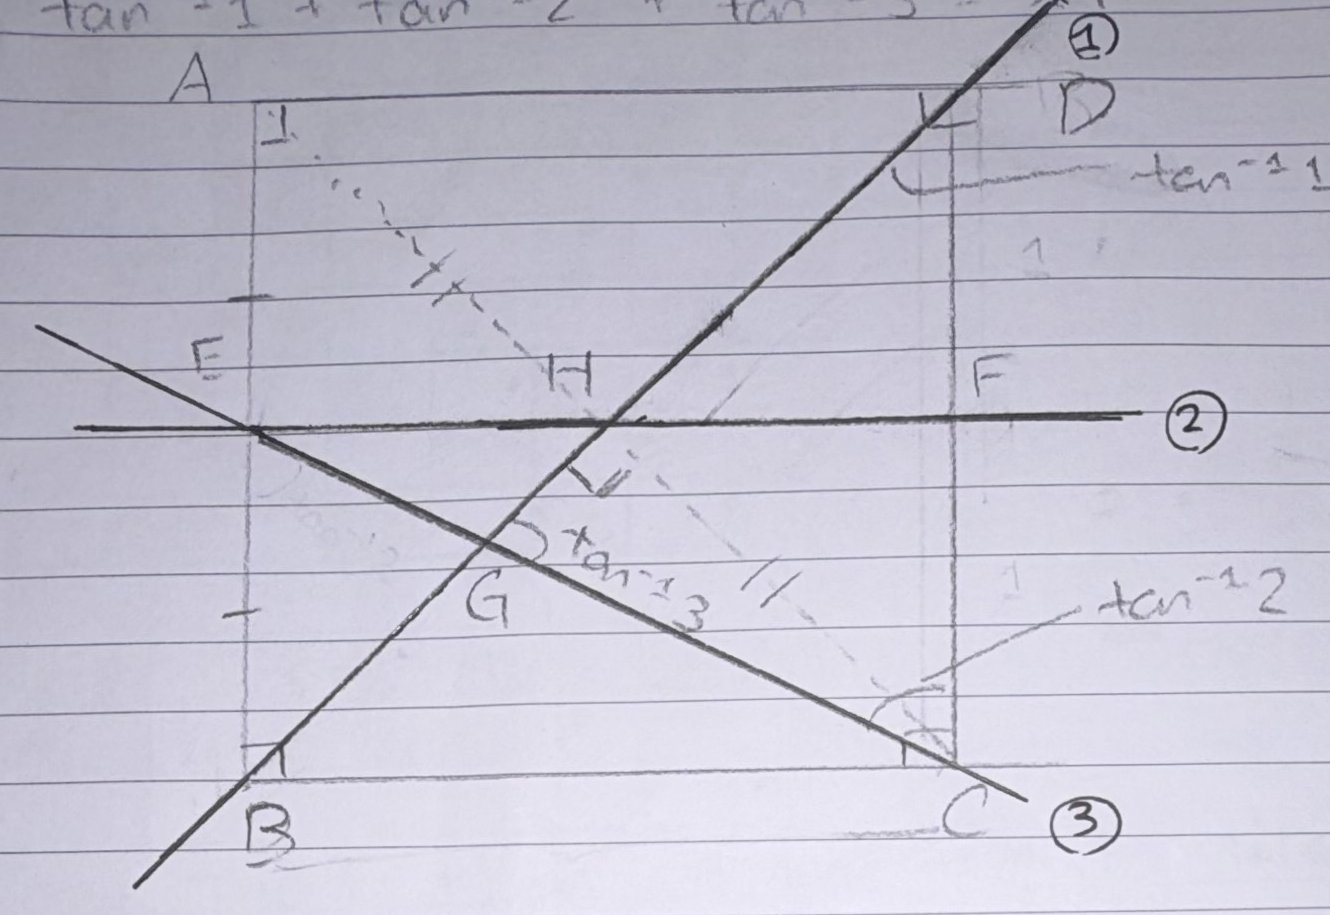
\includegraphics[width=0.6\textwidth]{figures/p2-fig-square.jpg}
\end{figure}

\noindent Notice that in $\triangle ABC$, $\overline{CE}$ and $\overline{BH}$ are the medians. Hence, their intersection, $G$, is the centroid, which divides $\overline{BH}$:
\[
    BG : GH = 2 : 1,
\]
or $BH = 3 \cdot GH$. Hence, as $CH = BH$,
\[
    \tan \angle CGH = \frac{CH}{GH} = \frac{BH}{GH} = \frac{3 \cdot GH}{GH} = 3.
\]
Hence,
\[
    \angle CGH = \tan^{-1} 3.
\]
Observe that
\[
    \angle BDC = \tan^{-1}\left(\frac{BC}{DC}\right) = \tan^{-1} 1
\]
and
\[
    \angle ECF = \tan^{-1}\left(\frac{EF}{CF}\right) = \tan^{-1} 2.
\]
As $\triangle GCD$ is a triangle,
\[
    \angle GDC + \angle DCG + \angle CGD = \tan^{-1} 1 + \tan^{-1} 2 + \tan^{-1} 3 = \pi. \qquad \square
\]

\section*{Acknowledgements / Transparency}

\begin{itemize}
    \item I wrote Problem 1 from memory, but it is not the most original problem -- it is a stock example in problem books which I do not think I took the time to develop in an unusually novel or clear manner.
    \item Problem 2 is from \textit{cut-the-knot.org} (Alexander Bogomolny).
    \item I used AI to help me typeset in order to save time.
\end{itemize}

\appendix

\section{Original Handwritten Working}

\subsection{Problem 1}

\begin{figure}[H]
    \centering
    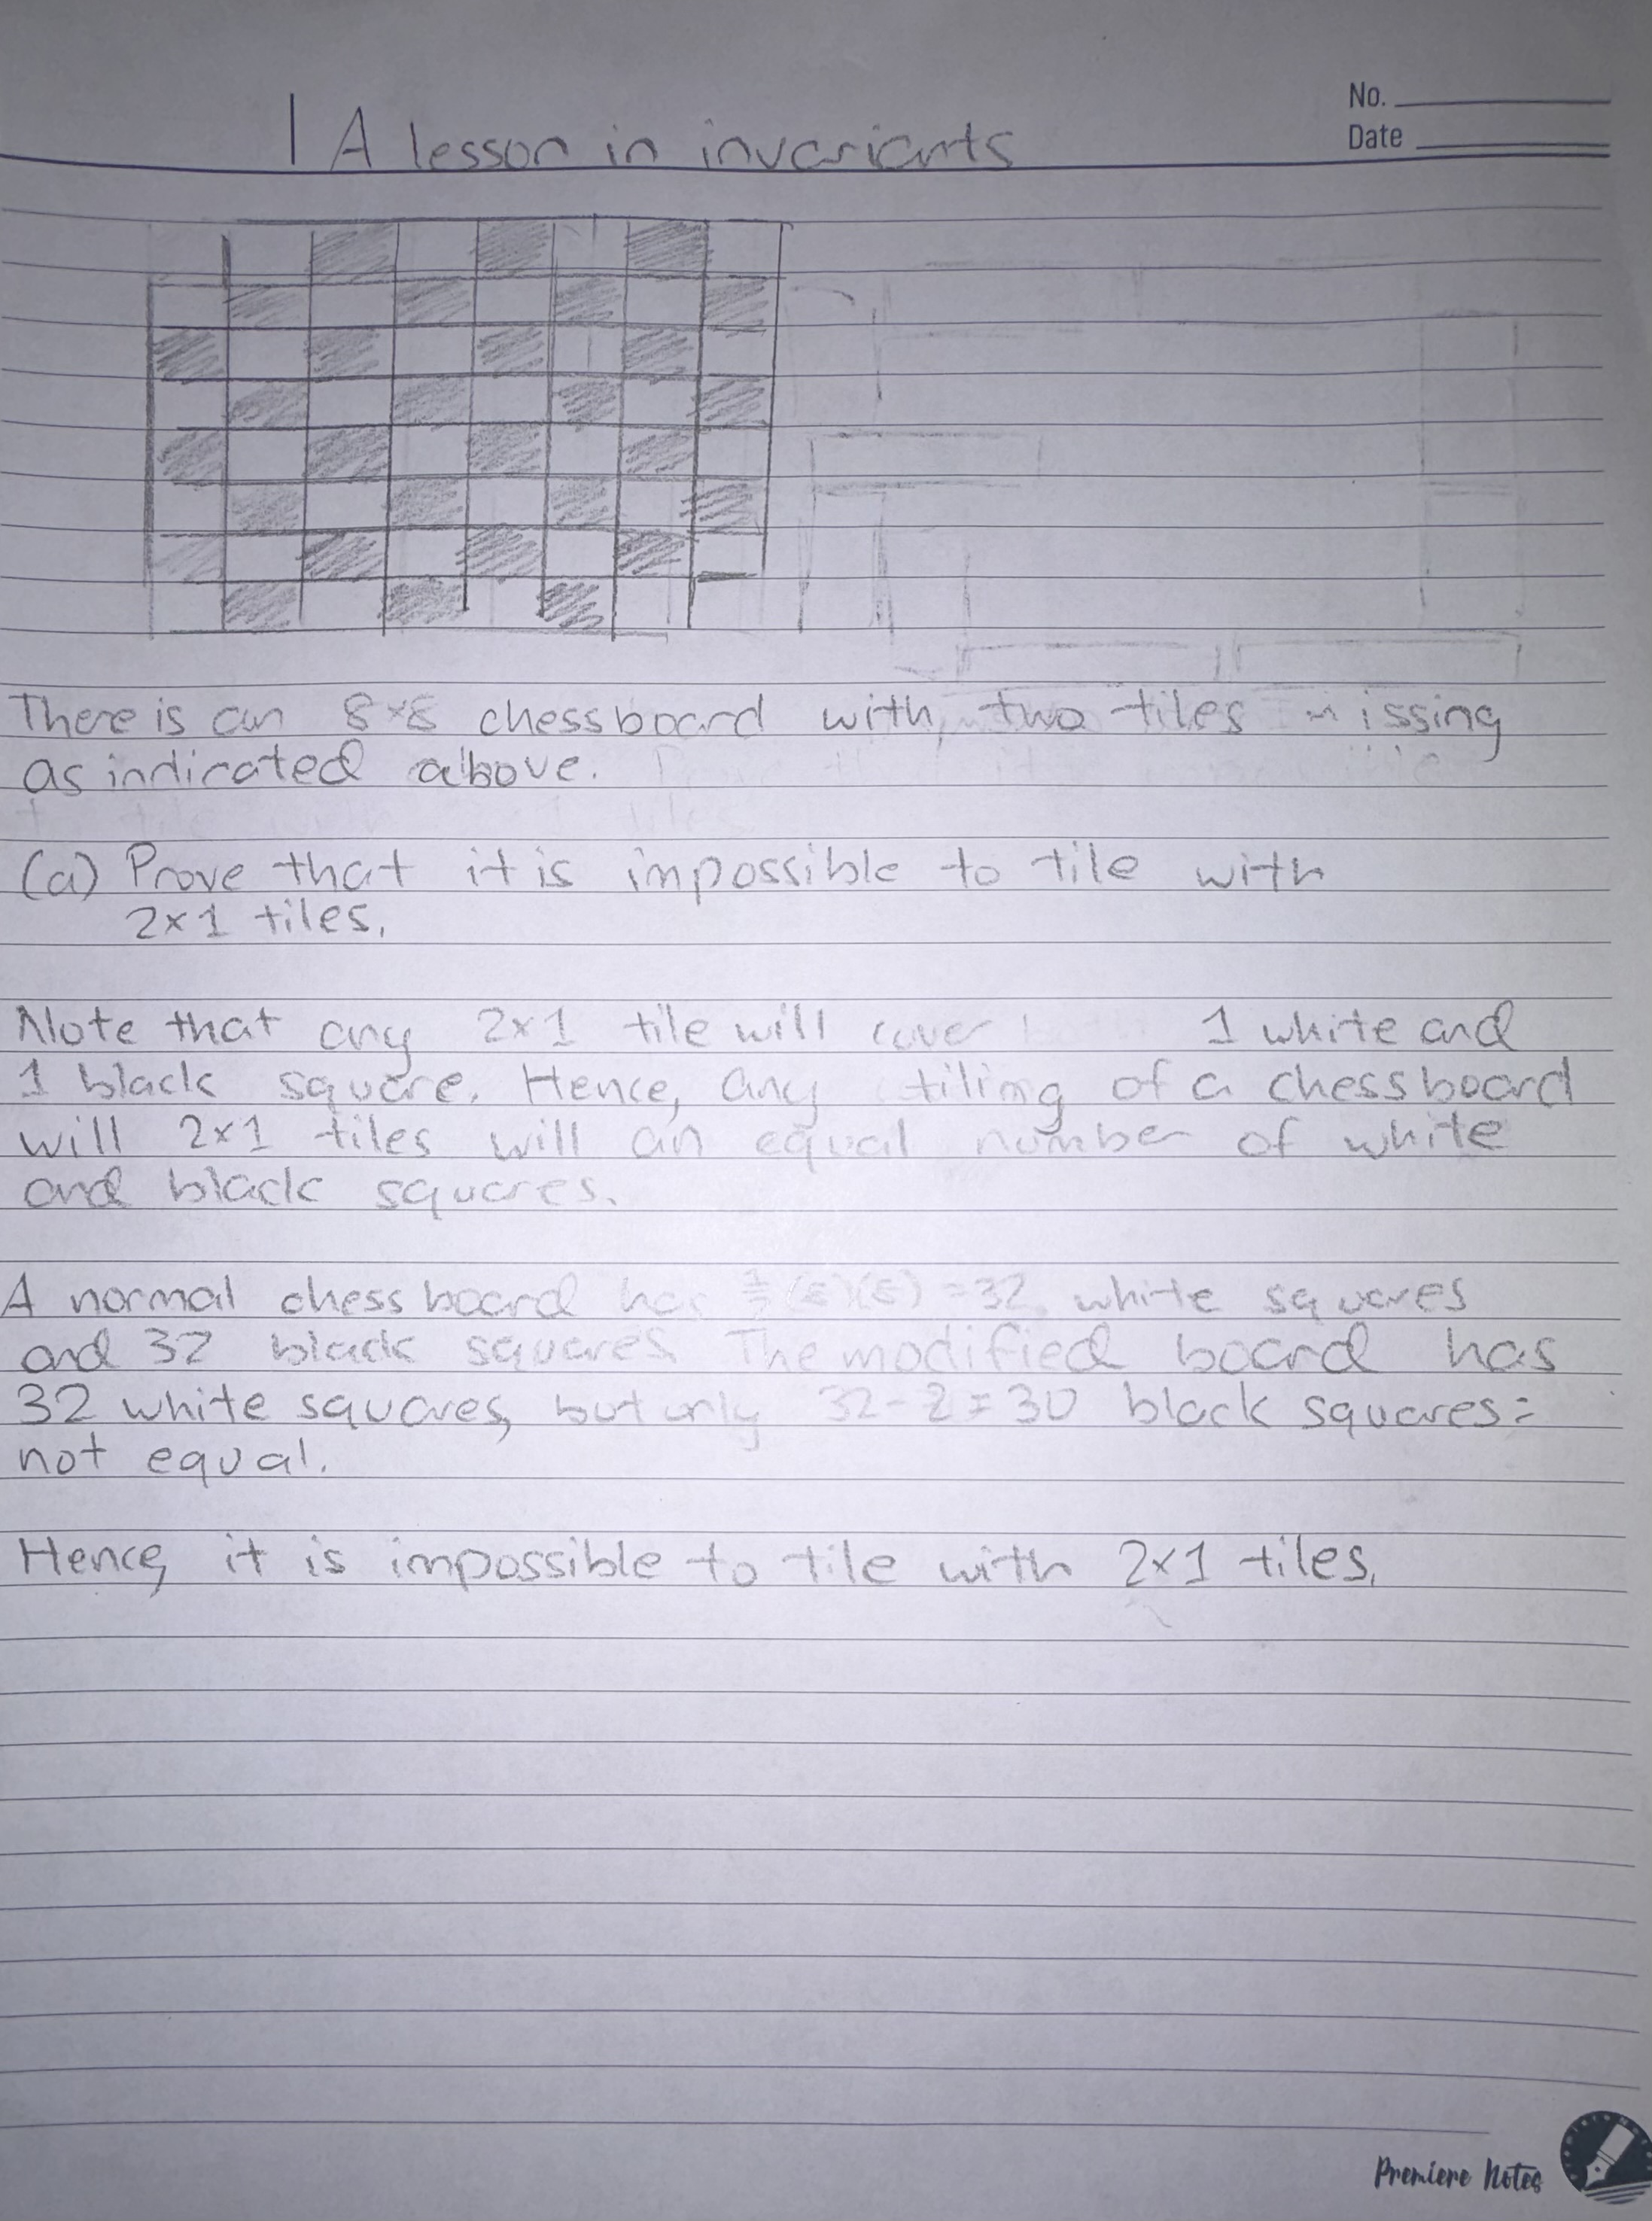
\includegraphics[width=0.6\textwidth]{figures/p1-page-1.jpg}
\end{figure}

\subsection{Problem 2}

\begin{figure}[H]
    \centering
    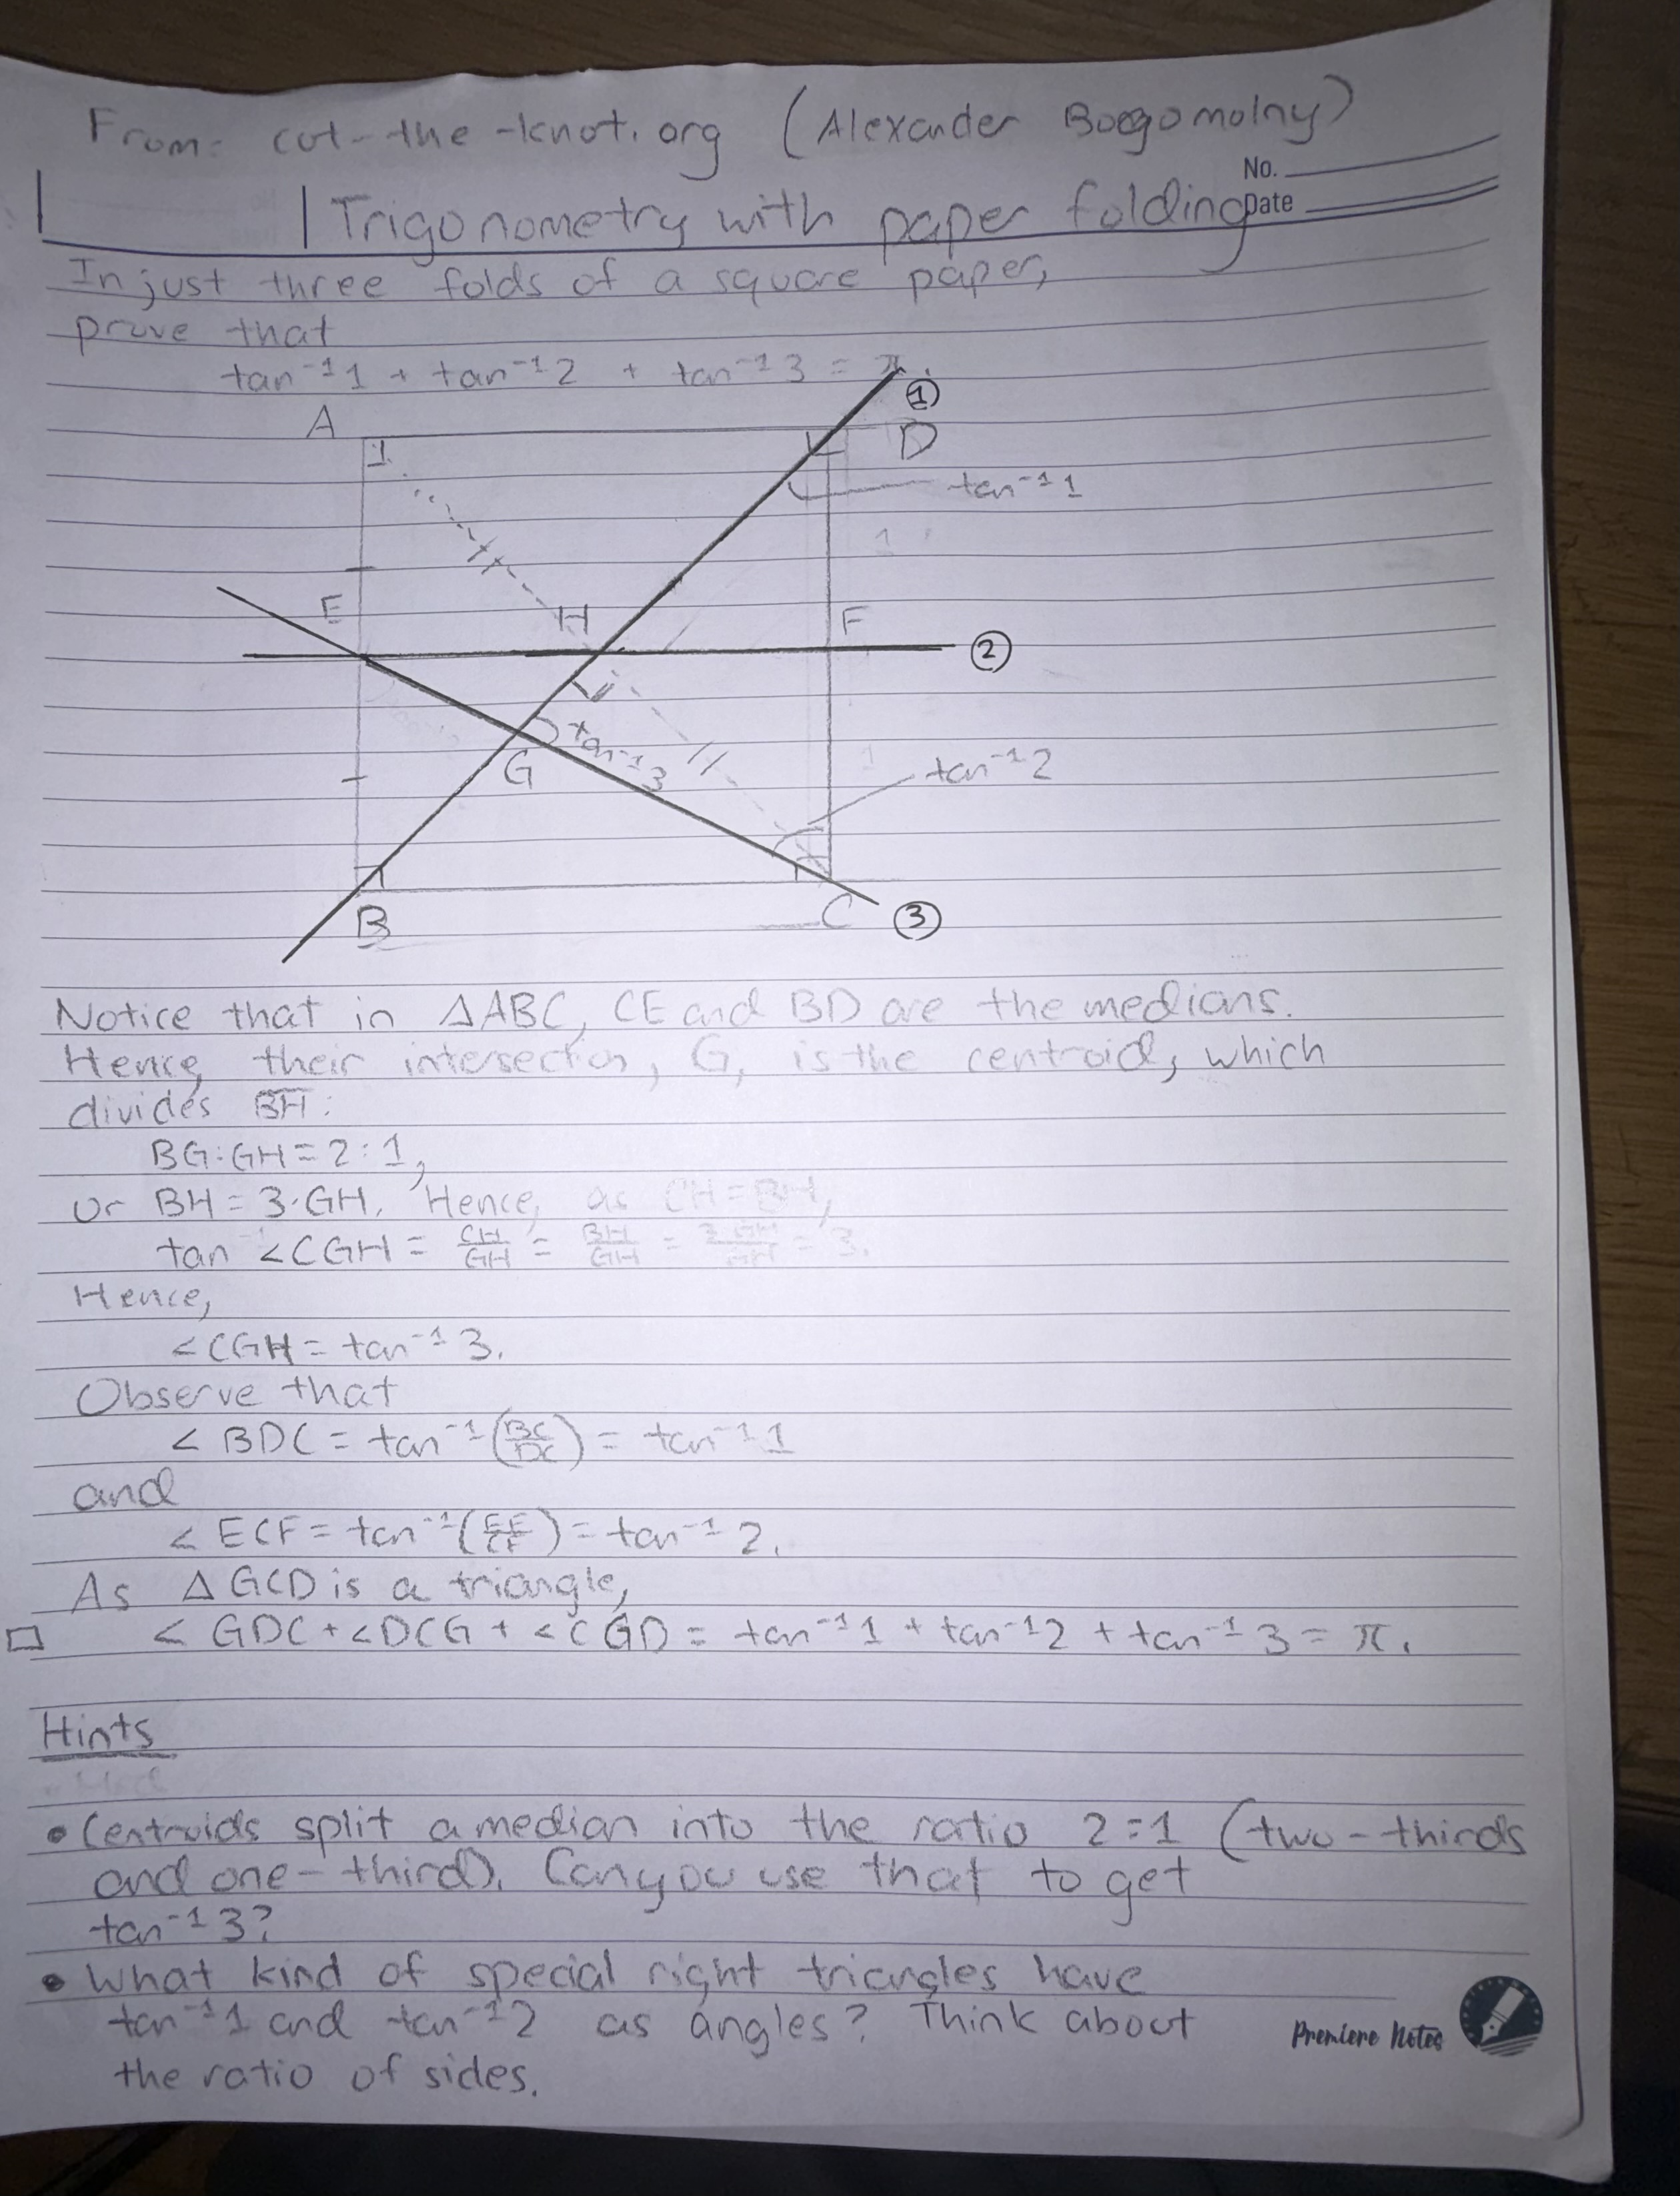
\includegraphics[width=0.6\textwidth]{figures/p2-page-1.jpg}
\end{figure}

\end{document}
